\chapter{Correlation Power Analysis} \label{c8_fifthcapter}

This lecture is the last technical lecture of the course about High Data
Complexity Power Analysis, CPA.

\section{Previous lectures recap}\label{c8_prev_lectures_recap:sec}

We are interested in laying a side channel attack. We got a device preforming
secret operation, AES operation. The device works as follows: we give input to
the device (plain text) and then it works on the input to produce an output
(cipher text) using a secret key. We want to recover the key. So, if we collect
many pairs of plain text and cipher text, what can we do with that? Lots of
things. In addition to plain text and cipher text, we have a side channel \cite{SideChannel}. What
is a side-channel? A side channel is an artifact of the computation and what's
nice about the channel is that it depends on the intermediate values of the
computation and not the output of it. We talked about number of side channels
throughout the course

\subsection{Timing side channel}\label{c8_prev_lectures_recap_timing_sc:subsec}

First, we used the time it took the computer to check for correct password in
order to find the password. Later, we used a timing attack \cite{TimingAttack} to attack RSA \cite{rivest1978method}.
Actually, we didn't attack RSA, we attacked an implementation of RSA which was
left to right multiplication exponentiation that uses a special representation
which is called Montgomery (the Montgomery basis). The Montgomery basis \cite{Montgomery}
representation which is very easy to do multiplications in this implementation,
almost as easy as doing regular multiplications, but there is a step called
Montgomery reduction which the computer does sometimes. Not a very expensive
operation but the computer only do it sometimes and because it does that that
sometime, in each encryption operation each exponentiation takes different time.
The time is a function of the plain text and the secret (in the case of RSA is
the private key). So how can we perform timing attack on RSA? We had a device,
the device got an input or message to sign and output the signed message and it
also outputted the time it took for the calculation. Our data structure had
plain text, signature(cipher text) and time.  The first step of the attack is to
take all the signatures and to throw them away. In the next step we tried to
guess one bit of the key. This guess helped us simulate a tiny little bit of the
secret operation, just one step and this step which we simulated. Since we
guessed the key, we could also guess this tiny step included a Montgomery
reduction. Our hypothesis is that if there is an extra Montgomery reduction, the
run time will be longer and if there is no Montgomery reduction the run time
will be shorter. Now we have a data structure: message and a bit, if the bit is
1 it means we think this was take longer and if it zero it means shorter. So, we
divided our set of traces into two groups, each one we gave a bit, 1 or 0. 

Now, how do we know that we guessed this bit correctly? We have in each row a
bit which says if we think it is longer or shorter and the time it took. The
hypothesis that we are trying to prove is that the messages that we marked with
1 are going to take a longer time to compute than the ones that we marked with
0. We have two sets of traces: the one which are marked as 0 and the one marked
as 1. Our hypothesis is that they take different time to execute. We test this
hypothesis using statistics. We can use student's T-test or we can just compare
the average. So we guessed a key bit, how many ways are there of guessing this
key bit? Two ways. So we have two hypothesizes, two proposed ways of splitting
our traces into two sets. In such a way, we can crack the key.

\subsection{Differential Power Analysis (DPA)}\label{c8_prev_lectures_recap_dpa_sc:subsec}

In DPA \cite{kocher1999differential, kocher1998introduction} the output of our device under test (DUT) is the cipher text. AES is a
very structured cipher, it has a fixed structure and it's going to be very rare
that we will have a different run time. So, usually there is a program running
on a CPU which has a clock and in each tick execute operation. AES is very
simple: it shifts, xor and so on. Luckily, we have other side channels, such as
current. The attacker took the device and measured the instantaneous power
consumption of the device. There are two ways for the attacker to do this. The
first way is to do this directly: take the current that is exiting the circuit
to the ground and instead of letting it go directly to the ground you send it
through a little probe, that will measure the power consumption on the circuit.
The advantage is that we get is a clean signal and the disadvantage is that we
will have to quite aggressively manipulate the device and maybe it's not a
reasonable assumption to make. The second way is electromagnetic (EM). What does
EM means? 

\begin{figure}[!ht]
    \centering
    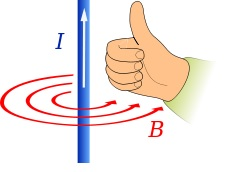
\includegraphics{images/chapter8/right_hand_rule.jpeg}
    \caption{Right hand rule} \label{c8_right_hand_rule:fig}
\end{figure}

Current (I) flowing through a wire and the change in the current generates EM
wave, so if we will put an antenna next to a wire we will be able to pick up the
current on this wire next to the antenna and to do this we only need to get
close (don't need to cut anything open), which makes it more reasonable attack
model. The disadvantages is that you have a lot of noise going on and you will
have a lot of RF signal processing to do so it's not trivial to get from there
to the key. Let's assume we are doing PA without EM. So, your output now is a
data structure. This data structure has plain text, cipher text and power
consumption, but power consumption is not a fixed value, it's a trace vector.
Now, if you think about device under test (DUT), most of the time when we are
doing the measurement of the power consumption it's not actually handling the
secret, it's doing something else. So if we look at the first byte of the key of
AES, its processed in the beginning of the encryption where there is adding the
key operation. The idea of AES is that every bit of the key will get mixed into
the whole cipher text, so it's not very easy to track it. In the beginning of
the encryption the key is not being processed at all and at the end its affected
so dilute into the cipher text. So there is going to be very specific time when
this trace is interesting. From a very long trace with millions of points there
are only few interesting points for an attacker. In DPA we had one number, the
time, and we knew that the signal was decoded in this number. Now we have a big
vector and we know the signal is somewhere in there but it's not in all of the
points. But we did the same thing here, we guessed a little part of key and then
we gave each one of the rows in the data structure a bit, one or zero. So, we
looked at some kind of intermediate value, we have the AES state and we took a
little bit of the state and we gave each one of the rows in the data structure
again, a one bit value and the one bit value was exactly the value of this bit
of the state. Actually we have a way of splitting our group of traces into two,
same thing as the timing attack. We claim that if we guessed the bit correctly
we just made a meaningful split of the traces. Now we divide our traces into two
sets and we want to test if there are different distributions. We hope that at
some point (the correct time) there will be a good distribution. An important
thing to understand is how many ways we have to split the traces into two in the
timing attack. If we guess one bit of the key, there are two ways of splitting.
Each time we decided we guessed a key bit we simulate it a little bit and then
we gave each entry in the data structure a value of 1 or 0. However, AES is a
byte oriented algorithm, so there is 256 ways of splitting, i.e. We have 256
different competing ways of splitting the traces into two. But again, we split
the traces into two. So, once we decide on a split we go over the data structure
and each row we assign a value of 1 or 0. Then we perform difference of means,
i.e. we take the mean of the right, the mean of the left and we have 256
different ways of splitting into two and look at the difference of mean where we
get the largest difference between the two means. 

\section{Correlation Power Analysis (CPA)}\label{c8_cpa:sec}

\subsection{Hamming weight}\label{c8_CPA_hamming_weight:subsec}

The hamming weight \cite{hamming} of a number is the amount of bits which are 1 in it's binary
representation. Hamming weight can refer to a hamming weight of state, or to
hamming distance, which means how many bits change between from one state to the
next. Lets assume we are looking at the hamming weight of a byte. This hamming
weight have values between 0 and 8. A number with hamming weight 0 will be 0 and
a number with hamming weight one will be 8, 2, 4. For $m$ independent and uniformly
distibuted bits, the whole word has an avergae Hamming weight $\mu_h = m/2$.

\subsection{CPA background}\label{c8_CPA_background:subsec}

We need to find a way to know when the traces are different. In DPA \cite{kocher1999differential, kocher1998introduction} we guessed
one byte of the key so we have 256 ways of splitting, but still, based on this
guess we only guess one bit of side-channel. So now we have 256 different ways
of splitting the cipher text into two groups and if we guessed right the two
groups will be different, but they will be different only at the correct time.
At previous lessons we learned that most computers these days are based on
technology called CMOS. The idea of CMOS is that if nothing much is happening,
if it's in a static state,  the power consumption is very low. But, if it's
dynamic, if it switches between 1 and 0, there are bursts of power consumption.
So, in a CMOS device the power instantaneous power consumption is correlated
with the amount of bits which are flipping in this time period. This fact was
completely ignored when we did DPA. We just said the power consumption was
different. As opposed to DPA, CPA doesn't ignore that fact. 

In CPA \cite{brier2004correlation, coron1962statistics, mayer2000smartly, oswald2003side},
we are going to guess one byte of the key, but we are not going to look
at one bit of the state but we are going to look at the hamming weight of the
state. Assume that if we guessed a byte correctly, the CPU is going to have to
handle a byte with it's hamming weight. For example, if we  guessed that the
state was 3, then the CPU will have to handle a byte with hamming weight of 2.
Our data structure is plain text and instead of a division to 0 or 1 we will
have a number between 0 and 8. This number is the hamming weight of the byte we
expecting the device to handle. Instead of splitting the trace into two groups,
we are going to use correlation. Due to CMOS, we can add a very reasonable claim
that when more bits are changing the power consumption raises.

\subsection{CPA on AES motivation}

AES \cite{anderson1998serpent} is byte oriented so we have 256 different guesses. Now, we are trying to
give label to each one of the inputs. We start with a guess and then we give it
a label. The first step of AES is to take the bytes of the plain text and XOR
them with the secret (bit wise operation). The next step is to apply the subByte
transformation, which is basically a look-up table. After applying subByte we
have a byte which is a mixture of the plain text that we know and the key which
is secret. So if we guess a key we can completely simulate the value. After
subByte we apply shiftRows. But shiftRows is just reading and writing the same
value from memory. It actually reading this value (HW(S[P xor K])) and make it
even stronger. Next there is Mix columns operation. The mixColumns operation
uses 32 bits so we will have 232 different guesses to do mixColumns. Since 232
is a low we will need a lot of traces and we will need to measure the DUT a lot
of times. Then we classify the measurements. There is going to be a statistical
meaningful classification for correct guesses. We refer readers to \cite{AESDescription} 
for a further detailed explanation of AES algorithm.

\begin{figure}[!ht]
    \centering
    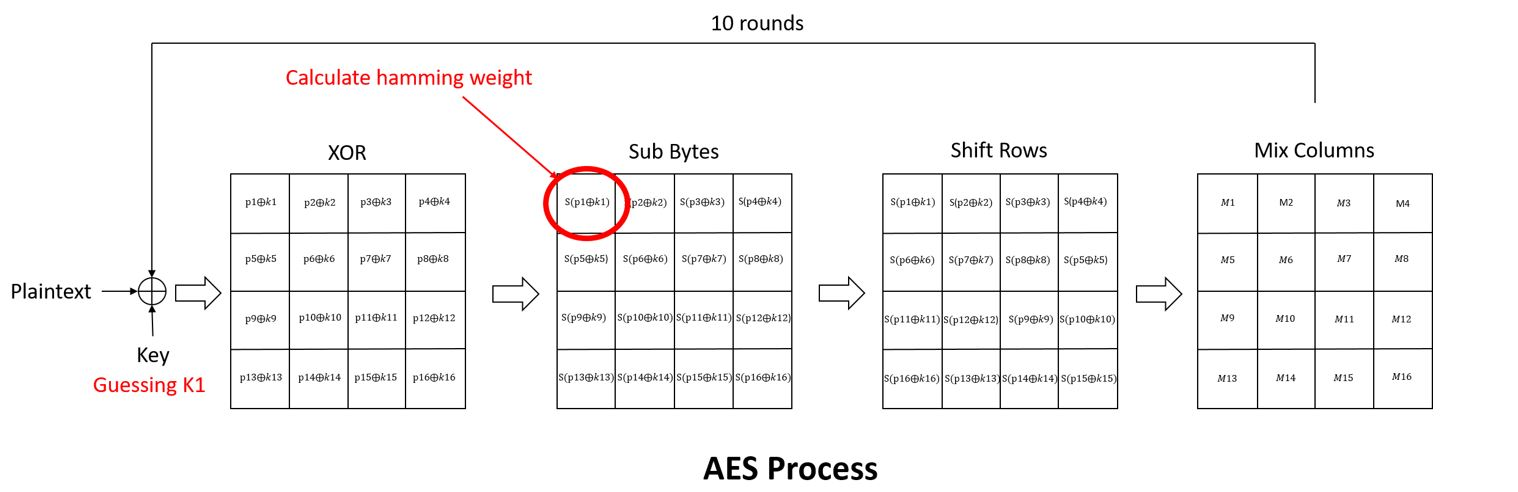
\includegraphics[width=1.0\textwidth]{images/chapter8/aes_process.jpg}
    \caption{AES illustration} \label{c8_aes:fig}
\end{figure}

In the timing attack days the meaningful was that we can run the students t-test
and get a division into 2 sets. In DPA we did  difference of means. To find
meaningful classification in CPA we will need the statistical Pearson
Correlation Coefficient~\cite{PearsonCorrelationCoefficient}. The Correlation
Coefficient is simply the covariance normalized to be between -1 and 1. The
intuition is that if the correlation coefficient is zero than it means we are
not guessing the key correctly and if we are guessing the key correctly we are
getting a correlation coefficient which is high, notably better than what we get
on the other key guesses. 

\subsection{CPA's data structures}\label{c8_CPA_data_structures:subsec}

When we were looking at a timing attack we had a data structure of size D, we
had D inputs, each input was a message we are trying to sign. To each of these
inputs we had a trace, our side-channel trace. The trace was a single number.
Our data structure was D times one. When we do High Data Complexity power
analysis we are going to do D different inputs, and each one of these lines
represent a single trace, i.e. long vector , and not a single point like the
timing attack. The vector with size T represents power consumption of the device
running a input in T different points of time. So we have a matrix data
structure of size D times T. D different inputs and T different times. Each line
of the matrix can be thought as if we fix the plain text and ask what the power
consumption over time of this plain text is.

Each column of the matrix can be thought as if we fix time and ask what is the
power consumption of the device in that particular time. One of these times
called the correct time, and we will get statistical meaning in that time. In
other incorrect times we won't get any statistical meaning because the DUT is
not processing the data we are looking at this particular time.

Note that in order that the CPA attack succeed, we have to align the traces to
the same time. Together with this matrix we have another data structure which is
the inputs, so each one of these lines says “this is the encryption of plain
text A, this is the encryption of plain text B” and so on. There are all sort of
ways of getting it, depending on the attack model. One way is that the attacker
has a signing oracle and the attacker chooses the plain texts and send them to
the device. This is the easiest model of the attack. Another way which is a
little more difficult is that the attacker has to commit ahead of time all the
plain texts and then the device encrypts them all at once, so he can't adapt to
whatever input he gives.

\subsection{CPA on AES step by step}\label{c8_CPA_overview:subsec}

We want to do a CPA of the AES encryption. We want to guess one byte of the key
and we want to get this byte mixed with the plain text which we know and we
don't want to many bits of the key to get mixed in because than we will have a
lot of guesses. So, the plain text comes in here and we know the plain text. We
mix it with the unknown key. The key is a guess. How many guesses are there for
the key?  $2^{128}$ ways of guessing the key. However in order to not guess the
entire key at once, we can guess only one byte at a time, so actually there is
256 guesses. 

For a key guess, We can simulate the key bit XOR plain text. Then, we can
simulate subByte of (key XOR plain text), and then we can also simulate
shiftRows on that result. This is where our simulation stops, because to
simulate mixColumns we need to guess 32 bits of the key and we don't want to
guess 32 bits. The trick is that when the DUT is manipulating this value (the
value we got after the simulation stopped), it will have some power consumption,
and that power consumption will be correlated to the hamming weight of that
value (according to the assumption we have on the CPA attack). 

Example: Let's assume we guessed the key byte as 5. So, if we know the guess of
the key byte is 5 we can look at the plain text and we know the first byte of
the plain text, so we can do key XOR plain text. We can do subByte of key XOR
plain text and we can calculate the hamming weight of it. So, we have a vector
of size D which is the hamming weight that we guessed for each one of the
inputs. We have a function which receives as input the plain text and our guess
and outputs the hamming weight. We have D different inputs, so we will call this
function D times, and will get an output of vector of size D. 

If we guessed the key correctly, at some point in time, which is called the
correct time, the power consumption will indeed be correlated (close to +-1)
with this vector that we guessed and all of the other times will not be
correlated (since the DUT is not only processing this byte of the key, but it is
processing other bytes of the key, other things and more). But in the correct
time there is going to be a correlation. If we didn't guessed the right key,
there will be no time which will have a correlation, meaning the correlation is
close to zero. If I say that there is a correlation, meaning the correlation is
close to +-1. 

\subsection{CPA warm up example}\label{c8_CPA_warm_up_example:subsec}

We have a DUT, we have a matrix of traces, we know the plain text, we know the
cipher text, we know the power traces and we know the key. So we have the power
trace and you want to find where inside the power trace is this bit being
processed. Our objective now is to find out when is the DUT processing the first
byte of the key. It could be interesting for us if you want to do fault attack \cite{FaultAttack}
or template attack \cite{TemplateAttack} or if you just want to make sure that you know how to do CPA.
As we saw earlier, the hamming weight of the subByte output is a good
hypothesis.

Now, let's look at our data structure. We have a matrix of traces, D time T.
Assume we have 1000 traces. Each one of these traces covers a long period of
time, several millisecond so it has 1 million points. Each one of these values
is not Boolean, usually it's one byte if you are using a regular source code. We
also have the inputs, we know for each one of these traces what was the plain
text being processed. The size of the plain text in AES is 16 bytes (128 bits).
So we have another data structure which is 128 bit by 1000 rows, so each input
is 128 bit has 1 Megabyte of a trace attached to it. We also know the key, so we
don't have to guess it. So now, we are trying to find out where is the correct
time. We want to find out for example, when is the DUT processing the first byte
of the key. So we go over each one of our plain text. We can do plain text XOR
key, we can also do subByte of that and we can do hamming weight of the output
of subByte. To each of the input plain text we associate the output hamming
weight. Our hypothesis is that the hamming weight the device will have to
manipulate is the output hamming weight we calculated. We created 1000 such
numbers. Each of the rows will now have plain text, trace, and hypothesis.

\begin{figure}[!ht]
    \centering
    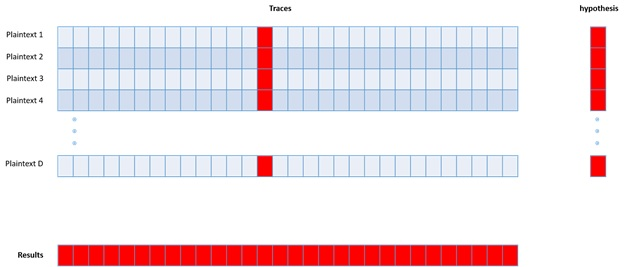
\includegraphics[width=1.0\textwidth]{images/chapter8/cpa_warmup_example.jpg}
    \caption{Graphic way of CPA warm up example} \label{c8_cpa_warmup_example:fig}
\end{figure}

The next step is to take the hypothesis and to sweep it across all moments of
time. Assume we have a fixed certain moment in time, i.e. a vector of size 1
time 1000. This vector is the instantaneous power consumption of the device at
the fixed particular time. Recall that the hypothesis is also a vector of size 1
time 1000. For 2 vectors of size 1000 we calculate the Pearson Correlation
Coefficient. The Pearson Correlation Coefficient function receives as an input 2
vectors of 1 by 1000 and outputs a single value between -1 and 1. If this value
is very high or low it means that there is a correlation between the input
vectors, but if it is close to zero it means there is no correlation between the
vectors. We will execute this process for each fixed moment in time, in our
example we will run in 1 million times. So the output of this step is a vector
of size 1 million by 1. So 1 million different times, for each one of these
times we have a single value between -1 and 1. Now we can look at this and see
where the maximum absolute valued point is and it is probably the correct time.

\subsection{CPA example}\label{c8_CPA_example:subsec}

However, in the warm-up example we had one assumption that not always correct -
we assumed we know the key. In the following example we want to do CPA in case
we don't know the key. We still have a matrix of traces. To each trace we have
the associated input plain text. In order to solve the key problem, we will run
the warm-up CPA 256 times. Each time we guess the key. If we are guessing the
key as 0 we will have a hypothesis vector and we can sweep it and get a vector
of million times one. We can also try key 1 and sweep it again and get another
vector. Also for key 2, key 3 all going to key 0xff, i.e. 256 different key
guesses, which gives us 256 times a million possible correlations. In this case
we have 256 guesses and not single hypothesis vector, but a hypothesis matrix.
256 different hypothesizes, each column in the hypothesizes matrix is like the
warm-up. Then we take this matrix and sweep it across this matrix. At the end we
get million different time by 256 different key guesses and each one of the
points in this matrix represents the correlation between our hypothesis and the
instantaneous power consumption of all of the devices at one particular moment
in time. So this is a two dimensional matrix and each row corresponds to a key
and each column corresponds to a time. So, most of the times, 99.9\%, this
matrix is going to be more or less 0. But there is going to be some points where
there is a good correlation, and this point are at the correct time and the
correct key!

Let's do this in pictures. So, when we had a single hypothesis we would take
this red row and we sweep it across this red line, this was the warm-up. But now
we don't know the key if it is red or blue or green, so we take this blue vector
and sweep it across and we will take this green vector and sweep it across. So
this is the output here, it has the same number of rows as the number of key
guesses and the same number of columns as we have times. This is full CPA and
hopefully in one of these rows we will have a peak and we will be happy. 

\begin{figure}[!ht]
    \centering
    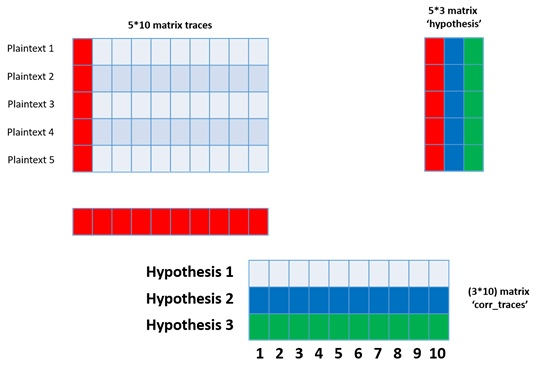
\includegraphics[width=1.0\textwidth]{images/chapter8/cpa_example.jpg}
    \caption{Graphic way of full CPA example} \label{c8_cpa_example:fig}
\end{figure}

\subsection{CPA in Matlab examples}\label{c6_Matlab_CPA_example:subsec}

We will show Matlab example which includes CPA, warm-up CPA, and the full CPA as
seen in this section. We are working on a data set called WS2 \cite{WS2} which is part of
the DPA toolkit. It has 200 traces, each one of size 30,000. These are power
traces of the first round of AES on an 8-bit micro-controller which is very low
clock speed and it's very vulnerable to DPA. In addition, that test setup is a
lab setup so this is the best we can hope for in terms of DPA. For each one of
the traces the plain text is known. \Cref{fig:c8_Matlab_power_as_sample_number}
describes the 200 traces power consumption as a function of the sample number. 

\begin{figure}[!ht]
    \centering
    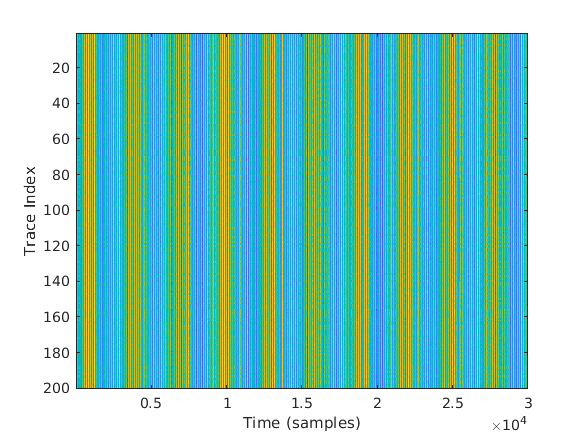
\includegraphics[width=1.0\textwidth]{images/chapter8/DataSet.png}
    \caption{Power consumption as a function of sample number} \label{fig:c8_Matlab_power_as_sample_number}
\end{figure}

The density of the colors indicates the instantaneous power consumption at a
particular moment at the DUT. The traces are very well aligned. Aligning is not
a simple task but this device was actually aligned. It was a lab setup so it is
easy to align. We can see that the device is doing the same thing at the same
time for all of these devices. If we will zoom in, we will see variation between
the traces. If we will zoom in to a two different traces, we will get figure
\ref{c8_Matlab_zoomin_on_two_traces:fig}.
\begin{figure}[!ht]
    \centering
    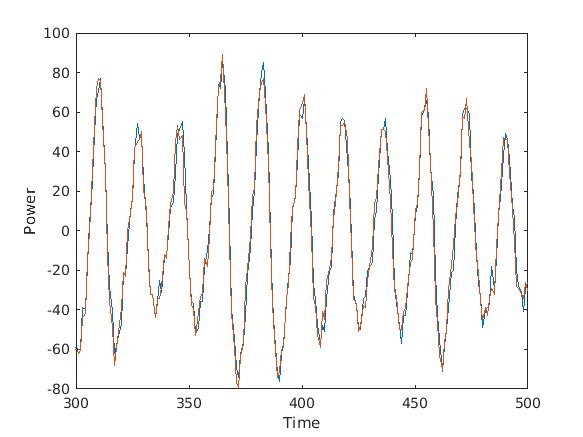
\includegraphics[width=1.0\textwidth]{images/chapter8/TwoSamples.png}
    \caption{Zoom-in on two different traces} \label{c8_Matlab_zoomin_on_two_traces:fig}
\end{figure}
The X axis represent the time (in samples) and the Y axis represent the power.
The power consumption is between +-80. These two traces are very similar but
there are some differences. The differences could be measurement noise or some
other signal processing.\\
For explanation let's do the warm-up example. At this example we know that the
first byte of the key is 120. Now that we know the key and the plain text we
could say that when we are at the correct time the DUT is going to be processing
a hamming weight of the correct key. In a DPA, first of all we find the plain
text XOR the key, at first we are looking only at the first byte, the result is
a number in the range of 0-255. Then we apply the AES subByte operation. Then we
are calculating the hamming weight of the outcome the values of the results are
between 0 to 8. By doing this we get the hypothesis\_vector for each particular
input.

\begin{figure}[!ht]
    \centering
    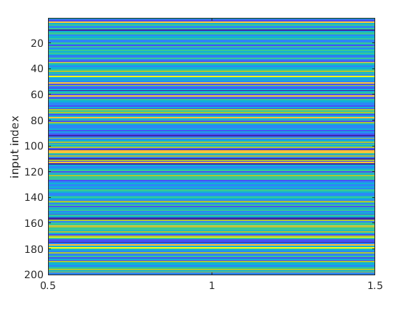
\includegraphics[width=1.0\textwidth]{images/chapter8/hypothesis_vector_values.png}
    \caption{Hypothesis vector values} \label{c8_Matlab_hypothesis_vector_values:fig}
\end{figure}


Figure \ref{c8_Matlab_hypothesis_vector_values:fig} presents the
hypothesis\_vector values (the X axis is not important). For each trace (Y axis)
we calculate the hamming distance (presented by different colors). Now that we
have figure \ref{fig:c8_Matlab_power_as_sample_number} and figure
\ref{c8_Matlab_hypothesis_vector_values:fig} we are going to sweep the later
figure over the former and for  each time we are going to calculate the Pearson
Correlation Coefficient. Thus, for each position we are going to get a number,
and this number will be between -1 and 1. Figure
\ref{c8_Matlab_pearson_correlation:fig} describes the results. 
\begin{figure}[!ht]
    \centering
    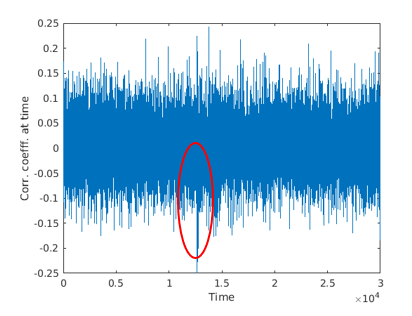
\includegraphics[width=1.0\textwidth]{images/chapter8/pearson_correlation_numbers.png}
    \caption{Pearson correlation graph} \label{c8_Matlab_pearson_correlation:fig}
\end{figure}
The X axis it the time in samples and the Y axis is the correlation Coefficient
between the hypothesis and the actual power consumption. Most of the time it's
around +-1 but there is a peak described by the red circle. This peak describes
the actual time that the AES making the sub byte operation on the first byte of
the key. 

However, this was the warm-up example. In a real attack scenario we don't know
the key. A real attack is very similar to the warm-up example, expect that we
are padding the key guessing by a loop and at this loop we are checking all the
256 available for the key. A real attack is described at figure
\ref{c8_Matlab_real_attack_scenario:fig}.
\begin{figure}[!ht]
    \centering
    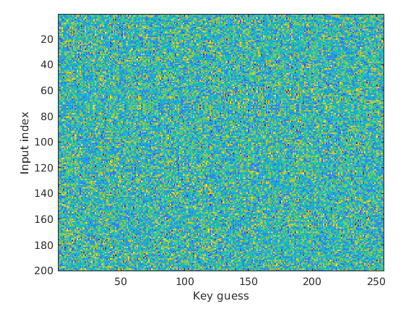
\includegraphics[width=1.0\textwidth]{images/chapter8/real_attack_scenario.png}
    \caption{Real attack scenario} \label{c8_Matlab_real_attack_scenario:fig}
\end{figure}

The X axis is time, and the Y axis are the key guesses. The color is the
correlation. Figure \ref{c8_Matlab_classification_matrix:fig} is the trace
classification matrix. The X axis is time, and the Y axis is the key guess. The
color is the correlation. From a first glance, the correlation is more or less
0. However, there is on this matrix one high value. If we will print out the
maximum of this matrix we will get 0.9168, which is very far from zero. 
\begin{figure}[!ht]
    \centering
    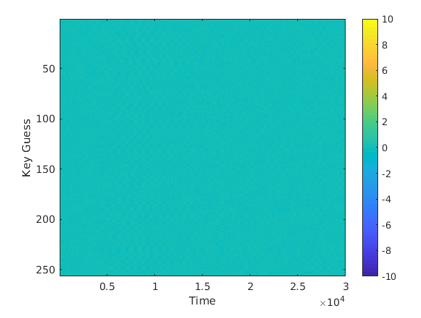
\includegraphics[width=1.0\textwidth]{images/chapter8/real_attack_classification_matrix.png}
    \caption{Real attack scenario classification matrix} \label{c8_Matlab_classification_matrix:fig}
\end{figure}

Now, we are going to find the correct time. The correct time is where there is a
maximum correlation and the correct key is the row number of this value. 
\begin{figure}[!ht]
    \centering
    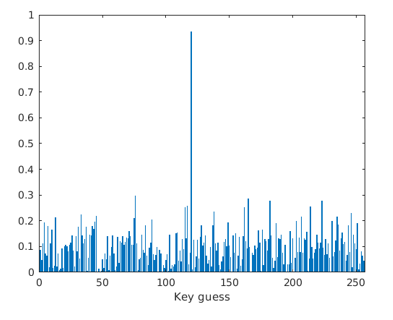
\includegraphics[width=1.0\textwidth]{images/chapter8/correct_time_graph.png}
    \caption{Correct time graph} \label{c8_Matlab_correct_time:fig}
\end{figure}
In figure \ref{c8_Matlab_correct_time:fig} we are taking the classification
matrix shown in \ref{c8_Matlab_classification_matrix:fig}  and we are looking at
the correct time. It has 256 different key guesses. The X axis is the key guess
and the Y axis is the correlation at the correct time. Most of the time the
correlation is around 0.3 but at the correct key guess the correlation is 0.9. 
\begin{figure}[!ht]
    \centering
    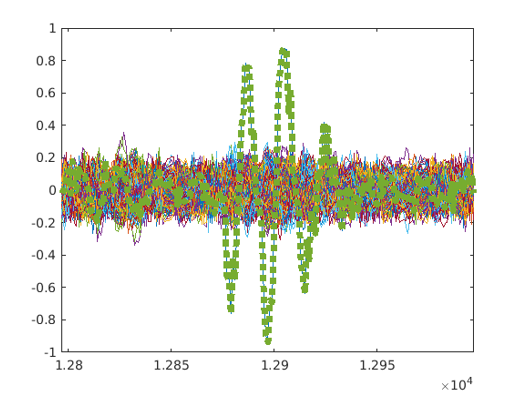
\includegraphics[width=1.0\textwidth]{images/chapter8/correlation_around_correct_time.png}
    \caption{Correlation around the correct time} \label{c8_Matlab_correlation_around_the_correct_time:fig}
\end{figure}

In figure \ref{c8_Matlab_correlation_around_the_correct_time:fig} we can see the
correlation around the correct time. The green line is the correlation for the
correct key guess, while the other lines are the correlation for the wrong key
guesses in the correct time.
\begin{figure}[!ht]
    \centering
    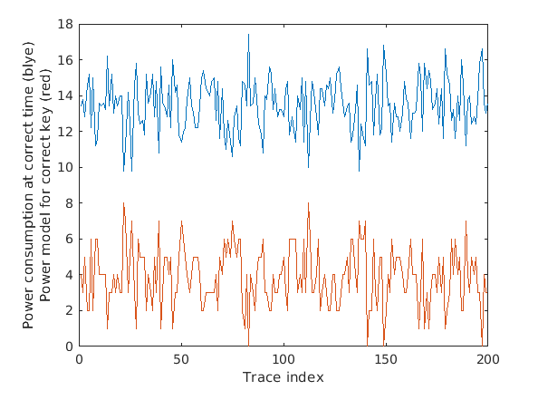
\includegraphics[width=1.0\textwidth]{images/chapter8/power_consumption_around_correct_time.png}
    \caption{Power consumption correlation around the correct time} \label{c8_Matlab_power_consumption_correlation_around_the_correct_time:fig}
\end{figure}
In addition, we can see in figure
\ref{c8_Matlab_power_consumption_correlation_around_the_correct_time:fig} the
real power consumption of the DUT vs. the hypothesis. The blue line is the power
consumption of the DUT at the correct time. The Y axis is traces. The red line
is the hypothesis that we tested. This two lines look correlated even to naked
eye, and it  is a negative correlation.